\documentclass{article}
\usepackage{graphicx} % Required for inserting images
\usepackage{hyperref} % Required for hyperlinks
\usepackage{amsmath}
\usepackage{multirow}
\graphicspath{ {./images/} }
\newcommand\tab[1][1cm]{\hspace*{#1}}
\title{Analyzing the Citation Rate of a Scientific Paper Using ML and Graph Algorithms}
\author{Vladimir Zakharov, Sergey Fedchin, Artem Chebykin}
\date{Fall 2024}

\begin{document}

\maketitle

\tableofcontents

\newpage
\section{Introduction}

\subsection{Paper Overview}

\tab Citation rate is an important metric to know about a scientific paper. It is often referred to as a KPI for researchers. Governmental agencies and scientists pay attention to the citation rate, when evaluating the quality of the paper. Hence, it is important to understand what exactly affects the citation of your work. In our research, we investigate the connection between various properties of scientific papers and their citation rates, using machine learning and graph algorithms. \\

\subsection{Field Overview}
\tab Due to the importance of citation rate prediction, there are quite a few papers on the subject, which implement various decisions of the stated problem. Those methods range from the most simple ones, which analyse the abstracts of papers with using just basic word embeddings; to a more complex, which take into account the structure of the citation graph. We will be using those simple models as a baseline for our own solutions, which will incorporate graph neural networks(GNN) in combination with the use of abstracts analysis. The studies, we have analyzed are: \\

\tab \href{https://link.springer.com/chapter/10.1007/978-3-642-40319-4_2?fromPaywallRec=false}{Predicting High Impact Academic Papers Using Citation Network Features} , that focused primarily on the graph features of the network, disregarding any meta-information about the paper, such as authotrs, scientific journal, which posted it, or even the abstract\\

\tab \href{https://link.springer.com/article/10.1007/s11192-020-03479-5?fromPaywallRec=true}{Predicting the future success of scientific publications through social network and semantic analysis} on the other hand, took into account the semantic structure of papers. However, this study used graph information only to create vertex features (betweenness, degree, etc.), and did not implement any graph ML approaches to perform the task\\

\tab \href{https://link.springer.com/chapter/10.1007/978-3-319-06483-3_4?fromPaywallRec=true}{Learning to Measure Influence in a Scientific Social Network} considered not only the author of a publication but also their co-authors, thus creating a more informative structure; yet only basic ML methods were used to conduct the research.\\

\tab If we want to talk about the use of papers abstracts, then \href{https://www.researchgate.net/publication/348440299_Citation_Intent_Classification_Using_Word_Embedding}{Citation Intent Classification Using Word Embedding} is the work to relate. In this study, a multitude of different models were used to create text embeddings for the papers, which were then used to predict citation rate by the paper abstract.\\

\tab The next paper inspired the way we interpreted the task, using older citation to predict the future ones: \href{https://www.researchgate.net/publication/381695536_Predicting_citation_impact_of_academic_papers_across_research_areas_using_multiple_models_and_early_citations}{Predicting citation impact of academic papers across research areas using multiple models and early citations}. The idea of splitting given graph by time, and using older and newer papers differently, as well as the use of a couple rather interesting ML algorithms, allowed authors to reach quite impressive results in terms of citation rate prediction .\\
\section{Data Acquisition and Preprocessing}

\tab	The amount of data and its quality is the basis for any data science research and there are quite a number of different datasets in this area. To explore the dependencies between the paper citation rate and its inner properties, we have chosen the dataset: \href{https://www.kaggle.com/datasets/wolfram77/graphs-snap-cit}{HepTh dataset} .The dataset represents the scientific paper citation graph in the field of high-energy physics in the years 1991 to 2003. There were 2 main reasons, for why this dataset was selected. Firstly, almost no research had been conducted on this data, which allowed us to implement baseline decisions from various other papers, and see how they perform on a different dataset. And secondly, due to limited resourses, we did not want to analyze extremely large dataset, so we needed something a touch smaller than that. \\

\tab	 Couple of words about the structure of the data. An oriented edge between vertices a$\rightarrow$b shows, that paper a cites paper b. Apart from the graph information itself, we are also provided with various features of each paper, which are, however, not standardized. Some features only appear in few papers, while others are present for each. We have decided to keep and work with the following features present for each paper: date of publication, authors, title + abstract. \\
\tab	The task of processing the dates was particularly tricky one since that part of the data was stored in a multitude of different formats, and they had to be standardized. (We have chosen yyyy-mm-dd format for it). Furthermore, the graph included some edges that led from an older paper to a more recent one, which didn't make sense; hence, those edges were removed from our data. We have also transformed the list of authors from a string into an actual Python list and parsed the abstract from the metadata files provided in the dataset. \\
\tab	After all the described manipulations, the data was ready for further exploration and analysis. \\

\section{Exploratory Data Analysis}
\tab All calculations with the graph were performed using \href{https://networkx.org/}{NetworkX} library in Python because it has a well-written documentation and provides a convenient interface.
\subsection{General Properties}

\tab Let $V$ be the set of all papers (nodes) and $E = \{(v_1, v_2): v_1, v_2 \in V, v_1 \text{ cites } v_2 \}$ all the citations between papers (directed edges). Then $G(V, E)$ is our directed citation graph.
For this graph $$|V| = 27,376$$ $$|E| = 351,025$$
\tab The original graph had more nodes -- 27.7K, but we discovered that it had around 140 weakly connected components (connected components in graph $G'$ obtained from $G$ by disregarding the edges orientation). Most of them were of sizes 3-5 so we decided to leave only the main component and delete all the stray nodes. Due to the graph's nature, it cannot be strongly connected (and number of strongly connected components is exactly $|V|$), since strong connectivity means that there exists a path from any node $v$ to any other node $u$ in the component, but it yields a cycle, which is impossible in G, as stated earlier. \\
\tab Some graph properties are defined for directed graphs only if they are strongly connected: diameter --- length of the "longest shortest path", average path length, girth -- length of the smallest cycle (usually only defined for undirected graphs). What we can calculate is the density of $G$:
$$D(G) = \frac{|E|}{2\binom{|V|}{2}} \approx 0.00046,$$
so the graph is rather sparse, which makes sense if we take into account the nature of $G$.\\
\tab One other characteristic that we can compute is the average clustering coefficient, which is a measure of the degree to which nodes in a graph tend to cluster together. 
$$\bar{C}(G) = \frac{1}{n}\sum_{v \in V}C_v \approx 0.156,$$
where $C_v$ is the local clustering coefficient of the node $v$, defined as $$C_v = \frac{|E(G(N_v))|}{\binom{V(G(N_v))}{2}},$$
if $G(N_v)$ is the subgraph of $G$ with only the immediate neighbours of $v$  as nodes.

\subsection{Degree Distribution}
\tab One of the important aspects of any graph is the distribution of the degrees of nodes. Since our graph is directed, we will have 2 distributions: one for the in-degree (number of incoming edges) and one for the out-degree (number of outgoing edges). Both of their distributions in log-scale are show on Figure \ref{plot:degree}.

\begin{figure}[h]
\centering
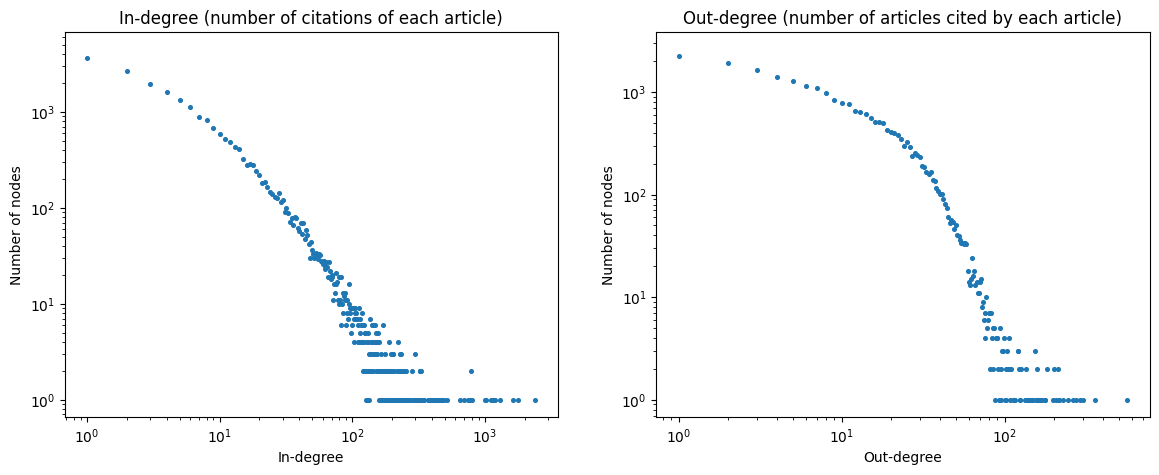
\includegraphics[width=1\linewidth]{degree_distribution.png}
\caption{Degrees distribution.}
\label{plot:degree}
\end{figure}

The first distribution is rather typical for a scale-free network and follows the power law. However, it is not exactly the case with the out-degree distribution. The possible explanation to this is the following: if we look at the graph as a temporal graph (we have dates of each paper's publishing) out-degree of each node is determined on creation and does not change over time. In-degree, on the other hand, has a behaviour that is much closer to how degrees act in a usual social graph, developing over time.

\subsection{Centralities}
\tab Centralities are characteristics of nodes that determine how "important" or "popular" each of them is. There are several types of them and each measures this "importance" in its own way. We will visualize distribution of three centralities.
\begin{itemize}
\item[a)] Eigenvector centrality. In general, relative scores are assigned to all nodes in the network based on the concept that connections to high-scoring nodes contribute more to the score of the node in question than equal connections to low-scoring nodes.
\begin{figure}[h]
\centering
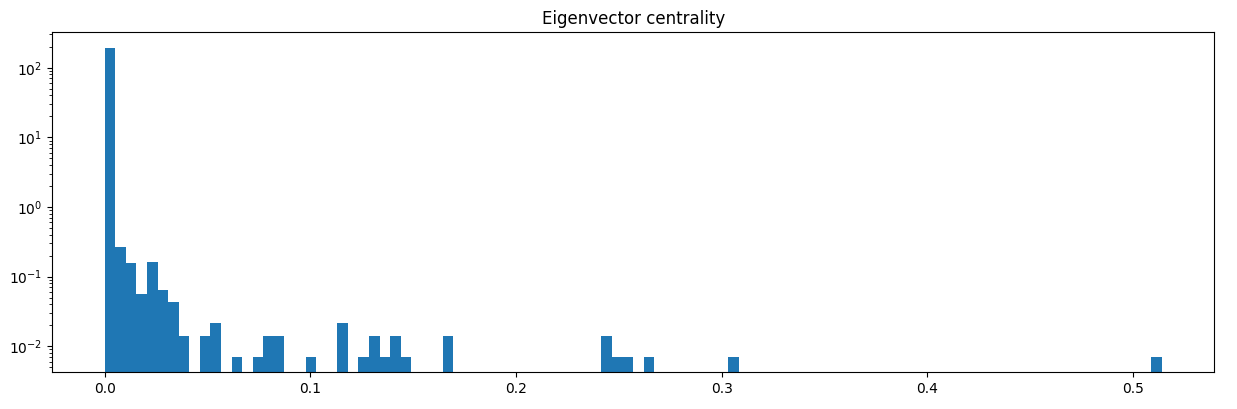
\includegraphics[width=1\linewidth]{centralities_eigenvector.png}
\caption{Eigenvector centrality distribution.} \label{plot:centrality:eigenvector}
\end{figure}
\item[b)] Closeness centrality. It is calculated as the reciprocal of the sum of the length of the shortest paths between the node and all other nodes in the graph. It measures how "close" the node is to the rest of the graph.
\begin{figure}[h]
\centering
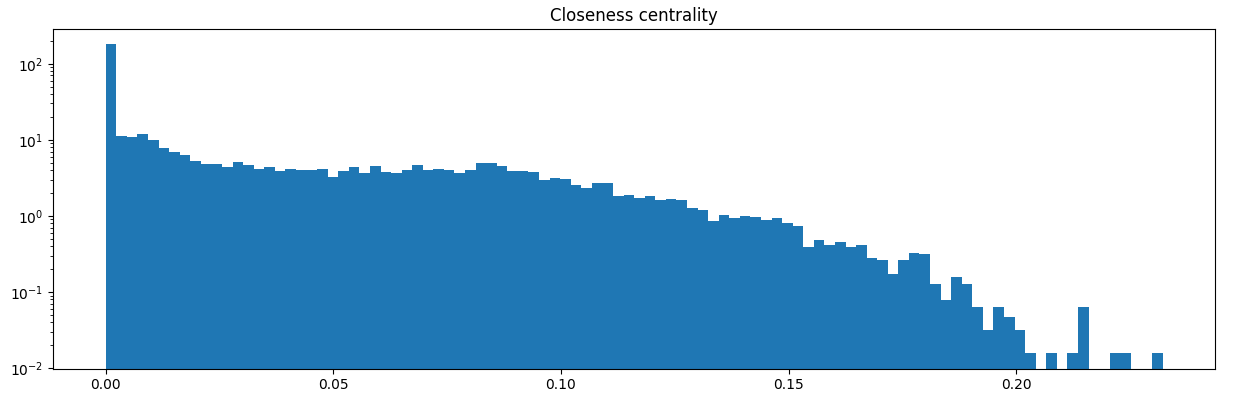
\includegraphics[width=1\linewidth]{centralities_closeness.png}
\caption{Closeness centrality distribution.} \label{plot:centrality:closeness}
\end{figure}
\item[c)] Betweenness centrality. The betweenness centrality for each node is the number of shortest paths that pass through this node. In other words, it determines whether the node is a hub.
\begin{figure}[h]
\centering
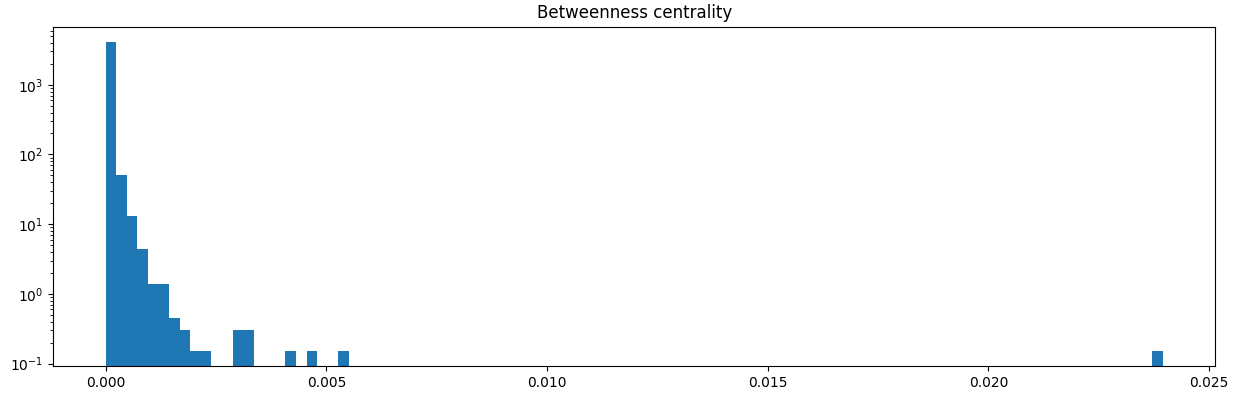
\includegraphics[width=1\linewidth]{centralities_betweenness.png}
\caption{Eigenvector centrality distribution.} \label{plot:centrality:betweenness}
\end{figure}
\end{itemize}

\subsection{Time Properties}
\tab Since our graph can be interpreted as a temporal graph, we can study the way its properties change over time. For instance, we discovered that the number of new papers per unit of time increases but the rate of the increase decreases. See Figure \ref{plot:number_of_new_papers} for the plots.
\begin{figure}[h]
\centering
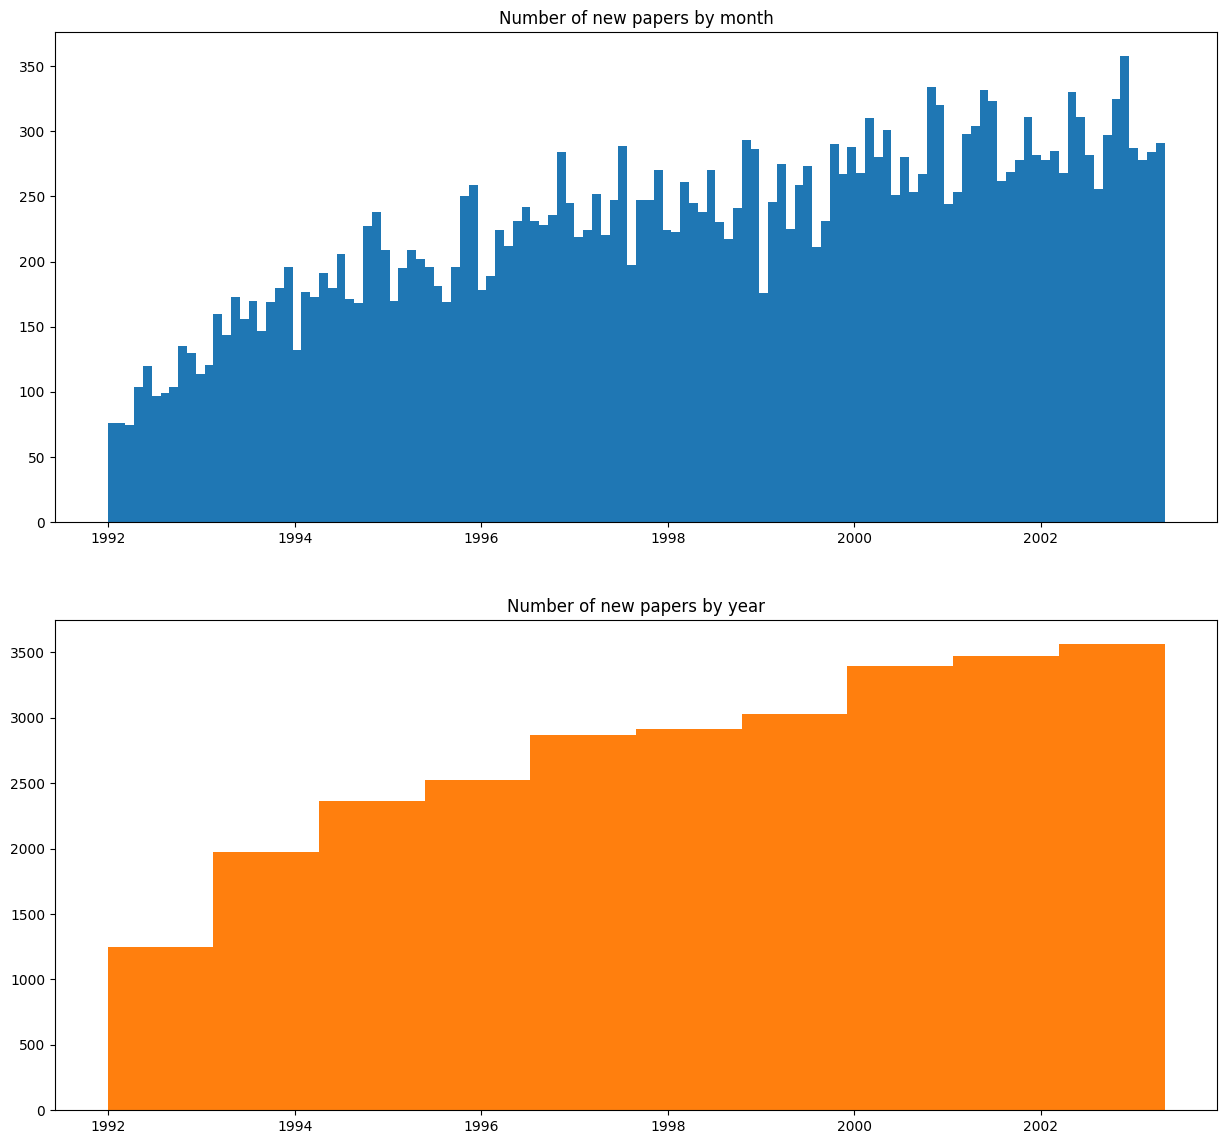
\includegraphics[width=0.9\linewidth]{new_papers_over_time.png}
\caption{Number of new papers published each two months and each year.}
\label{plot:number_of_new_papers}
\end{figure}

Another interesting thing that we found is how average in-degrees and out-degrees change (see Figure \ref{plot:average_degree_per_month}).
\begin{figure}[h]
\centering
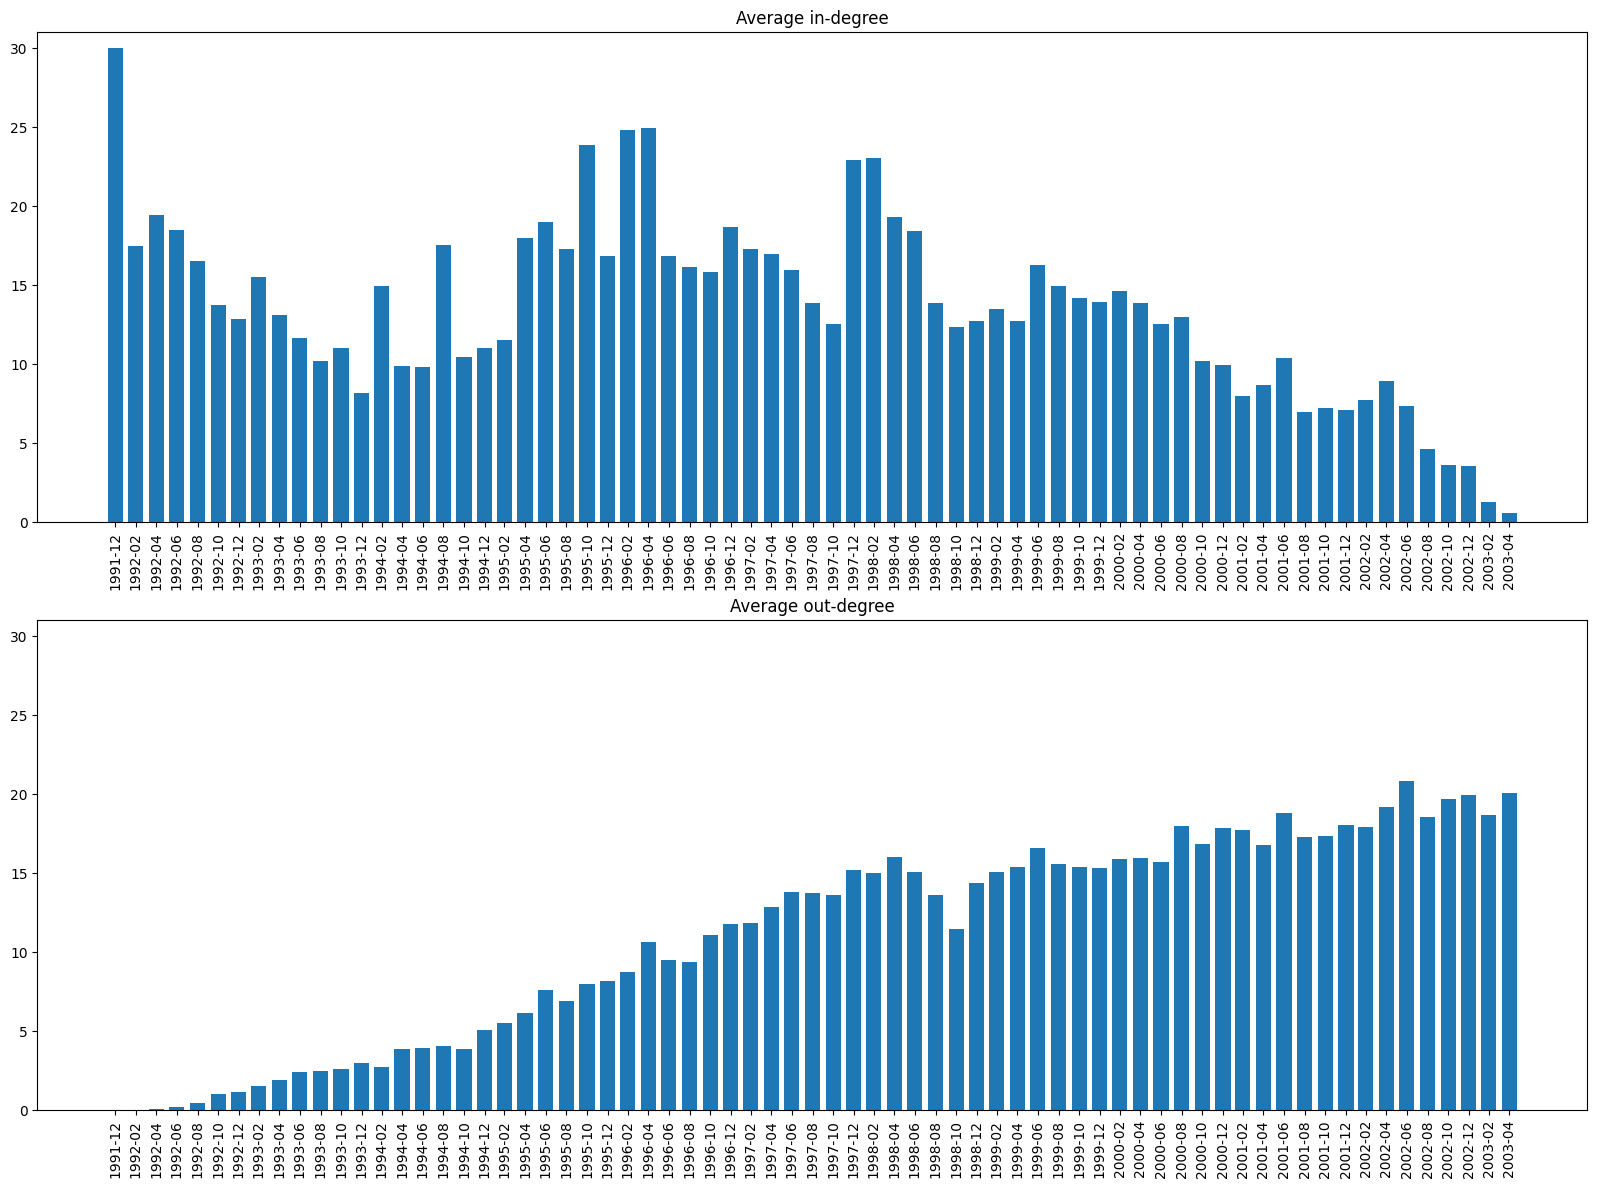
\includegraphics[width=1\linewidth]{degrees_over_time.png}
\caption{Average degrees in 2 months time from 1991 to 2003.} \label{plot:average_degree_per_month}
\end{figure}
A downwards trend in the end for in-degree and upwards trend in the beginning are noticeable. Explanation to this phenomena is rather simple: older papers had more time to gain popularity and therefore have more incoming edges, whereas papers from 2003 do not have any papers in our dataset that cite them. The opposite happens with the out-degree. Earlier papers cited even earlier papers (from 1980s) that were not included in our graph and thus have little to no outgoing edges. It is also worth noticing that the growth of out-degree slows down closer to 2003. It means that almost enough papers are included in the graph at that time to publish a paper sourcing only these modern papers in our dataset.

\subsection{Clusterization}
Due to the duality of our problem, clusterization can be done either using node features (mainly papers' abstracts) or considering the graph structure (which is usually called community detection). As a measure of quality of the partition $P$ of graph $G$ we have chosen the metric modularity, which for directed graphs is defined as
$$\textbf{Modularity}(G, P) = \frac{1}{|E|} \sum_{u, v \in V} \left[\left(A_{u, v} - \frac{d_{\text{out}}(u)\cdot d_{\text{in}}(v)}{|E|}\right)\cdot \delta_P(u, v)\right],$$
where $A$  is the adjacency matrix and $\delta_P(u, v)$ is defined as
$$\delta_P(u, v) =
\begin{cases}
1, & \text{if nodes } u \text{ and } v \text{ lie in the same community in pratition } P \\
0, & \text{otherwise}
\end{cases}.
$$ 

First we did community detection on the graph. We compared Louvain and label propagation community detection algorithms since most other methods were extremely slow and thus not suitable for our graph. The best modularity was achieved by Louvain algorithm with partition into 31 classes with fixed seed compared to 969 classes using label propagation. 

To do clusterixation we have divided the articles into the same number of clusters according to their abstracts using text embedding from `glove-wiki-gigaword-50` model (we averaged the embeddings of each word in the abstract) and KMeans algorithm. We also tried agglomerative clustering and Gaussian mixture. Modularity for all of them was really poor, which should not come as a surprise. Visualizations of resulting clustering can be found on Figures \ref{plot:clustering:agglomerative} and \ref{plot:clustering:gaussian_mixture}. The comparison of clustering algorithms can be seen in Table \ref{table:clusterization}.

\begin{figure}[h]
\centering
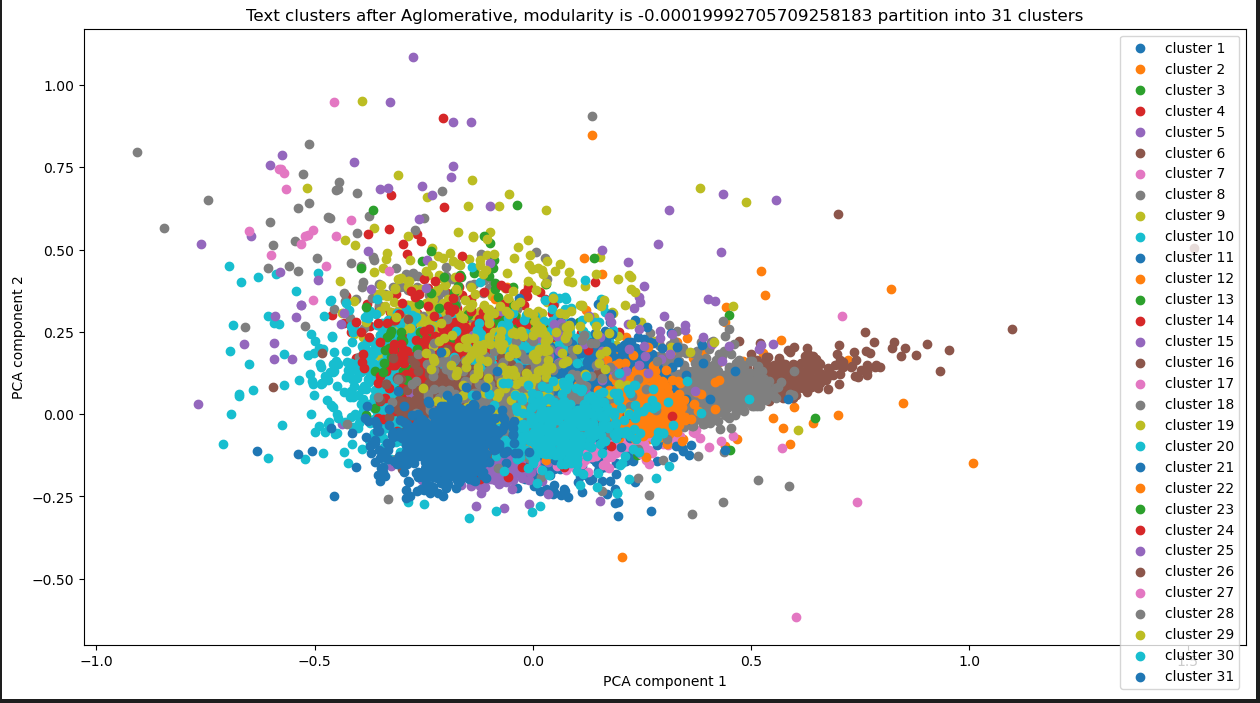
\includegraphics[width=1\linewidth]{Aglomerative.png}
\caption{Visualization of clustering using Agglomerative Clustering algorithm.}
\label{plot:clustering:agglomerative}
\end{figure}

\begin{figure}[h]
\centering
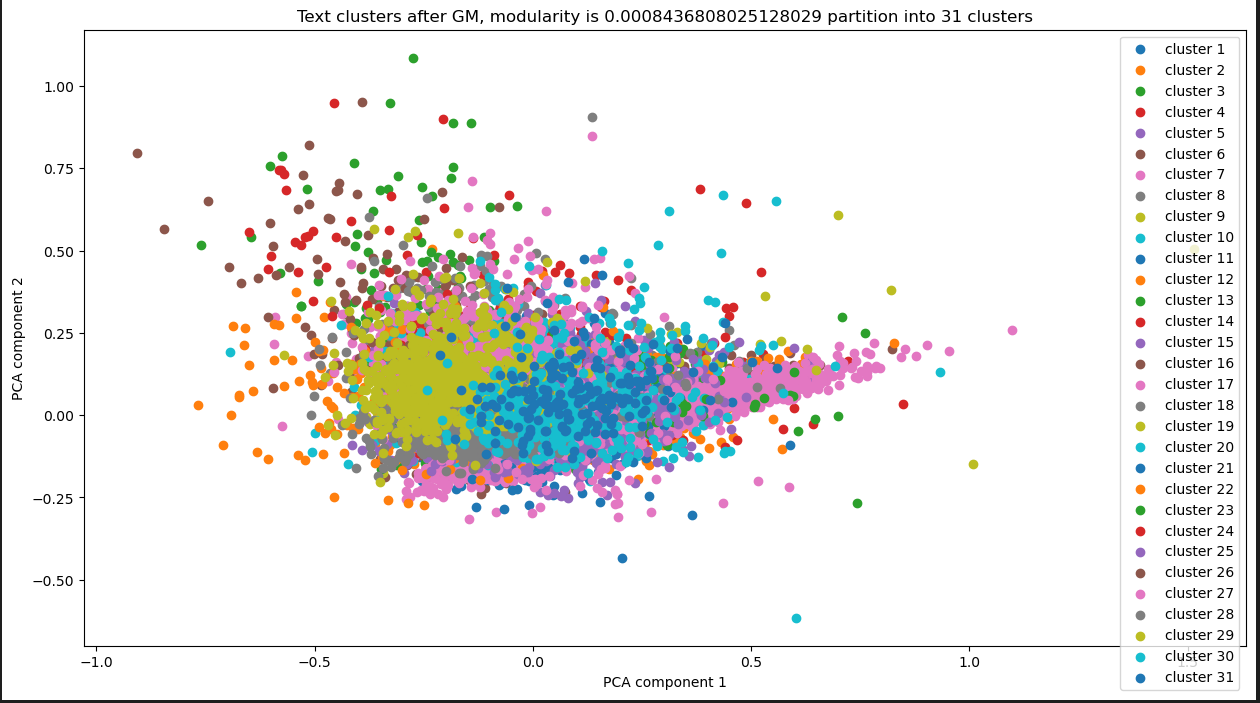
\includegraphics[width=1\linewidth]{gm.png}
\caption{Visualization of clustering using Gaussian Mixture model.}
\label{plot:clustering:gaussian_mixture}
\end{figure}

\begin{table}[h]
\centering
\begin{tabular}{c c c}
\hline\hline
Algorithm & Number of clusters & Modularity \\
\hline
Louvain & 31 & $0.655$ \\
Label Propagation & 969 & $0.541$ \\
Agglomerative Clustering & 31 & $-0.0002$ \\
Gaussian Mixture Model & 31 & $0.0008$ \\
\hline
\end{tabular}
\caption{Comparison of different clusterization algorithms.}
\label{table:clusterization}
\end{table}

\section{Methodology}
\subsection{Problem statement}
\tab Our main goal was to predict citation rates of the papers. We initially thought of solving a link prediction task (predicting the existence of edge between two nodes) since it seemed logical enough for our task. However, upon further considerations we eventually switched to node classifications. We classified citation rates into 4 classes using quartiles of in-degrees (this manner was inspired by scientific journals' tiers). This approach gave us even-ish distribution of classes. Note that the class boundaries are not evenly distributed, since our graph is a scale-free network.

To form target values and split our graph into train and test samples the following approach was used. Split the graph into two parts: all the nodes with publish date before 2001-01-01 (the date choice was arbitrary) and the rest of them, which will be referred to as old nodes and new nodes respectively. The new nodes have some edges into the old ones (new papers citing old papers), the number of which (converted into a class) for each old node was used as its target value. Note that the edges between old nodes were not considered in the target. By splitting old nodes into train and test sets we got our final data.

\subsection{Baseline}
\tab Before implementing any baseline we studied how other papers approached this problem. The state-of-the-art approach for baseline solutions, is to use some embedding method in combination with a simple regression or classification model(depending on the task). We used similar approach in out study

As a baseline model we employed logistic regression classifier as a classical model. We trained it on three different node embeddings:
\begin{enumerate}

\item[1.] Text embeddings. \newline
We tried two different approaches of getting text embeddings:
\begin{enumerate}
\item[a)] Text had been preprocessed using stemmer and stop words removal before applying bag of words vectorization.
\item[b)] Text embeddings were obtained by averaging the embedding of each word in the abstract using glove-wiki-gigaword model with an embedding size of 50
\end{enumerate}

\item[2.] Graph embeddings.\newline
We used the classic node2vec with default parameters, except that the dimension of the embedding space was 64 (instead of default 128)
\end{enumerate}

The results of these methods can be found in the Table \ref{table:baseline_metrics}

\begin{table}[h]
\centering
\begin{tabular}{c c  c c c}
\hline\hline
 & & \multicolumn{3}{c}{Metrics} \\
\cline{3-5}
Classification model & Embeddings & \multirow{2}{*}{Accuracy} & \multicolumn{2}{c}{F1 score} \\
 & & & Macro & Weighted \\
\hline
\multirow{3}{*}{Logistic Regression} & Text preprocessing + BoW & 0.46 & 0.38 & 0.45 \\
 & Text 2 & 0.44 & 0.16 & 0.27 \\
 & Graph & 0.53 & 0.33 & 0.43 \\
\hline
\end{tabular}
\caption{Baseline metrics.}
\label{table:baseline_metrics}
\end{table}

\subsection{Our solution}
In search of a better solution, we tried GCN and GCNwLinear models with different types of node embeddings: random embeddings (learnable), text/graph-only embeddings and their concatenation (we tried using each of them separately, as well as in combination with each other). In addition, we went through the following parameters:
\begin{verbatim}
n_layers = 6
random_emb_size = 32
hidden_dim = 128
crop_df = False
tune_embs = True
add_reverse_edges = True
dropout=0.2
lr = 5e-4
node_emb_size = 64
\end{verbatim}
Each parameter speaks for itself except of \textbf{crop\_df} which is responsible for getting rid of the imbalance of classes in the dataset by removing some samples or not. Above, is the best subset of these hyperparameters, we were able to find for GCNwLinear model, which uses combination of text and node embeddings. The metrics achieved by this model are shown below:
\begin{table}[h]
\centering
\begin{tabular}{c c  c c c}
\hline\hline
 & & \multicolumn{3}{c}{Metrics} \\
\cline{3-5}
Classification model & Embeddings & \multirow{2}{*}{Accuracy} & \multicolumn{2}{c}{F1 score} \\
 & & & Macro & Weighted \\
\hline
\multirow{1}{*}{GCNwLinear} & Concatenated text and node embs & 0.58 & 0.54 & 0.59 \\
\hline
\end{tabular}
\caption{Final metrics.}
\label{table:final_metrics}
\end{table}
\section{Conclusion}
\tab Unlike the other works, we implemented the combination of text embeddings and node embeddings to complete the task of predicting citation rate. As we can see, on the chosen dataset, this method performed better than other methods from previous works on this subject. Not only were the metrics improved, but also the balance of predicted citation rates became better, not ignoring or overemphasizing any particular class. This goes to show, that GNN models have a bright future regarding the task of predicting citation rates.
As per usual, those models should be tested more on different datasets and different areas of scientific publication, to confirm its effectiveness and achieve better results.
\end{document}